%=======================================================================
% IEEE CONFERENCE paper -- BLINDED SUBMISSION COPY (ICOSICS 2026).
% This file is IDENTICAL to main.tex except: (1) the author block is
% replaced with the standard IEEE double-blind placeholder, and (2) a
% short AI-assistance disclosure statement is added before the
% bibliography, per the venue's ethics policy. Use THIS file for the
% initial double-blind submission; use main.tex (named authors) for the
% camera-ready version after acceptance.
%
% Compile on Overleaf: pdfLaTeX, run twice + BibTeX.
%=======================================================================
\documentclass[conference]{IEEEtran}
\IEEEoverridecommandlockouts

\usepackage{cite}
\usepackage{amsmath,amssymb}
\usepackage{graphicx}
\usepackage{booktabs}
\usepackage{url}
\usepackage[table]{xcolor}
\usepackage{tikz}
\usetikzlibrary{shapes.geometric,arrows.meta,positioning}
\usepackage{pgfplots}
\pgfplotsset{compat=1.17}
\usepackage{algorithm}
\usepackage{algorithmic}
\usepackage[hidelinks]{hyperref}

\newcommand{\ph}[1]{{\color{red}\textbf{[#1]}}}

\begin{document}

\title{A Hybrid Rule--Transformer Web Application Firewall\\
with Inline Blocking and False-Positive-Controlled Fusion}

\author{\IEEEauthorblockN{Anonymous Author(s)}
\IEEEauthorblockA{Affiliation withheld for double-blind review}
}

\maketitle

\begin{abstract}
Most web application firewalls still lean on signature matching, and that
approach breaks down fast against obfuscated payloads. Transformer-based
detectors have been proposed as a replacement and look impressive on paper,
but the papers reporting those numbers almost never place the model inline,
measure its latency, or ask what it costs in false positives. This paper
does. We built a WAF that runs a fine-tuned transformer inside a real Nginx
\texttt{auth\_request} enforcement path, governed by a four-tier
rule--model fusion policy, and tested the whole system end to end on
CSIC~2010. The BERT detector alone reaches F1~$0.966$ at a $4.4\%$
false-positive rate (ROC--AUC~$0.986$), which beats a signature engine
outright ($0.567$ F1) and edges past a strong TF--IDF baseline while adding
only $12.0$~ms of median GPU inference latency. Here is the part we did not
expect: both the model alone and the full rule-plus-model hybrid survive all
six semantics-preserving evasion techniques we tried---$0\%$ evasion either
way. That means adversarial mutation is not what justifies the hybrid's
higher false-positive rate ($23.1\%$ vs.\ $4.4\%$). What does justify it
only shows up once you leave the training distribution: tested zero-shot on
an unrelated corpus, SR-BH~2020, the model alone collapses to FPR~$1.00$,
while the hybrid still holds at F1~$0.971$. We report this as it
happened---an accuracy, robustness, and generalisation trade-off, not a
clean win for either design.
\end{abstract}

\begin{IEEEkeywords}
web application firewall, transformer, BERT, inline enforcement, decision fusion.
\end{IEEEkeywords}

\section{Introduction}
Web applications are still the easiest way in. SQL injection, cross-site
scripting, path traversal, and command injection keep showing up at the top
of the OWASP Top Ten year after year, and the standard defence against them
is a web application firewall (WAF): an intermediary sitting in front of the
application, inspecting every request, and blocking whatever looks
malicious before it reaches the backend. For two decades that inspection has
mostly meant signatures and regular expressions---ModSecurity paired with
the OWASP Core Rule Set~\cite{owaspcrs} is the obvious example. Rule sets
like this are fast, auditable, and easy to reason about, but their weakness
is that they match surface syntax, not intent. Insert an inline comment,
flip the case of a few characters, chain a couple of URL encodings, and a
payload that means exactly the same thing to the backend no longer matches
the rule. Tighten the rules to catch that and you start blocking legitimate
users instead. Modern applications built around single-page front ends and
constant background polling only make this worse, since there is simply
more unusual-but-harmless traffic for the rules to misjudge.

Transformer language models~\cite{vaswani2017attention,devlin2019bert} are
the obvious next step: instead of enumerating every way an attack payload
might be spelled, let the model learn what malicious structure actually
looks like. On paper this works well---recent work reports accuracies above
$99\%$ for transformer-based web attack classifiers on the CSIC~2010
benchmark~\cite{wadbert2026,liu2024bertlstm}. But almost all of that work
stops at offline classification: train on a static corpus, report an
accuracy figure, done. Whether the detector could actually run as a
firewall is rarely asked. Three questions in particular go unanswered.
How much latency does the model add once it sits in the synchronous path of
every request? What false-positive rate does it impose on real users at a
chosen operating point, as opposed to a raw accuracy figure that says
nothing about that cost? And when it is combined with the rule-based
detection that is already deployed, does that help or hurt, and by how much?

This paper answers those three questions by building the thing and testing
it end to end rather than offline: a WAF in which a fine-tuned transformer
is a working component of a live inline enforcement path. Specifically, we
contribute:
\begin{itemize}
\item a transparent inline architecture built on Nginx's
\texttt{auth\_request} mechanism, adjudicating every request before it
reaches the backend without any modification to the protected application;
\item a four-tier decision-fusion policy that combines deterministic
signatures and anomaly rules with confidence-banded transformer scoring,
together with an endpoint-aware relaxation rule and a fail-open safeguard;
\item a full empirical evaluation---detection quality against baselines, an
ablation isolating what the rule layer actually contributes, a
threshold-sensitivity sweep, measured inline inference latency, and an
adversarial-evasion test comparing the model alone against the
hybrid---covering exactly the operational measurements the offline
literature tends to skip;
\item a cross-dataset generalisation test showing where the rule layer's
false-positive cost is actually earned back. It is not adversarial evasion,
where the model alone already matches the hybrid; it is zero-shot transfer
to an unfamiliar corpus, where the model alone falls apart and the hybrid
does not, giving an explicit accuracy--robustness--generalisation
trade-off rather than an unqualified accuracy claim.
\end{itemize}

\section{Related Work}
A recent survey situates transformers and LLMs for intrusion
detection~\cite{kheddar2025survey}. Rule sets such as OWASP CRS~\cite{owaspcrs}
are the practical baseline but match surface strings; classical ML on
CSIC~2010~\cite{payloadml2024svmrfxgb} depends on handcrafted
features. Recent deep and transformer detectors report $>$99\% within-corpus
accuracy for SQLi/XSS~\cite{scireports2024novelxsssqli,liu2024bertlstm,wadbert2026},
with enhanced neural architectures~\cite{zhou2025ewebguard} and BERT applied to
intrusion detection~\cite{yang2025bertids,sdnbert2024}; domain encoders such as
SecureBERT~\cite{aghaei2022securebert,aghaei2025securebert2} and compressed
variants such as DistilBERT~\cite{sanh2019distilbert} address inference cost.
Adversarial evasion remains open: the canonical WAF-A-MoLE
attack~\cite{demetrio2020wafamole} showed ML-based WAFs can be mutated past,
recent work crafts adversarial SQL injections against real-world
WAFs~\cite{advsqli2024}, uses reinforcement learning to craft evasive
payloads~\cite{mlwaf2025peerj}, and uses a generative LLM to synthesise XSS
payloads and blocking rules~\cite{genxss2025}, yet transformer-WAF
papers rarely test evasion. Across this work, inline deployment, latency,
false-positive control and cross-dataset generalisation are addressed rarely and
never jointly---the gap we close (Table~\ref{tab:survey}). Concretely: within-corpus
accuracy is reported repeatedly~\cite{scireports2024novelxsssqli,liu2024bertlstm,wadbert2026,zhou2025ewebguard},
but almost none of these studies place the trained classifier behind a real
reverse proxy, measure the added latency of that placement, or report what
happens to precision when the model is combined with (or substituted for) a
conventional rule layer under an explicit false-positive budget. Adversarial
robustness is evaluated even less often, and where it is
evaluated~\cite{advsqli2024,mlwaf2025peerj} the target is typically a
non-transformer classifier rather than a fine-tuned language model. This paper
is deliberately narrower in scope than a pure accuracy benchmark: it reports a
full deployment-oriented evaluation --- architecture, latency, ablation,
threshold sensitivity, and evasion --- on a single encoder, and treats the
resulting accuracy--robustness trade-off as a finding to be reported honestly
rather than optimised away.

Two design choices separate this work from the surveyed systems specifically.
First, several within-corpus studies~\cite{scireports2024novelxsssqli,liu2024bertlstm}
report accuracy at or above $99\%$ on CSIC~2010 without describing how the
train/test split was constructed; CSIC~2010's benign traffic is templated, so
a split that does not deduplicate near-identical benign requests before
partitioning permits leakage between train and test, which can inflate
reported accuracy without a corresponding improvement in real generalisation.
We deduplicate before splitting for this reason, which we believe is also why
our absolute F1 sits below those figures rather than above them. Second, work
that does evaluate adversarial robustness against WAF-style
detectors~\cite{advsqli2024,mlwaf2025peerj} targets classifiers other than a
fine-tuned transformer, so the extent to which a language-model-based
detector resists semantics-preserving mutation is comparatively unstudied;
our evasion results speak to exactly that gap, for the specific mutation
families we test.

\begin{table}[t]
\centering
\caption{Representative recent work vs.\ this paper.}
\label{tab:survey}
\footnotesize
\begin{tabular}{@{}p{2.2cm}p{0.6cm}p{1.7cm}p{2.2cm}@{}}
\toprule
Work & Year & Approach & Gap for WAF use \\
\midrule
WADBERT~\cite{wadbert2026} & 2026 & Dual-channel BERT & Offline only \\
BERT--LSTM~\cite{liu2024bertlstm} & 2024 & BERT+LSTM & Single class; offline \\
E-WebGuard~\cite{zhou2025ewebguard} & 2025 & Neural arch. & No inline/latency \\
Payload ML~\cite{payloadml2024svmrfxgb} & 2024 & SVM/RF/XGB & Handcrafted; offline \\
AdvSQLi~\cite{advsqli2024} & 2024 & Adv. SQLi & Attack; robustness open \\
\textbf{This work} & -- & Hybrid, inline & --- \\
\bottomrule
\end{tabular}
\end{table}

\section{System Architecture}
The WAF is a reverse proxy in three containers: an Nginx edge proxy, a detection
service (rules + transformer), and the unmodified backend
(Fig.~\ref{fig:arch}). Nginx's \texttt{auth\_request} turns every request into an
internal sub-request to the detection service, which replies \texttt{200}
(allow) or \texttt{403} (block); enforcement is inline and no request reaches the
backend before adjudication. The detection service applies four tiers: (1)
unambiguous signatures after double URL-decoding; (2) anomaly/injection rules;
(3) transformer scoring; (4) fusion (Algorithm~\ref{alg:fusion}).

Two policies temper the pipeline in deployment. A safelist of internal
endpoints---static assets, real-time channels such as WebSocket polling, and
framework routes---is evaluated only against the Tier~1 direct signatures, so the
high-volume, structurally unusual but benign traffic these endpoints generate is
not subjected to the anomaly rules or the model; this removes a large source of
false positives without materially widening the attack surface, since such
routes rarely carry user-controlled injection surface. Second, any unhandled
exception in the detection path---a malformed header, a model-loading failure, an
inference error---causes the service to fail open, returning an allow decision so
that a fault in the WAF cannot take the protected application down with it.
Fail-open is the correct default for an availability-critical middlebox, but it
is a security budget whose activation rate should be monitored in production.

\textbf{Threat model.} We assume an external, unauthenticated attacker who can
send arbitrary HTTP requests to the protected application and whose goal is
either a successful injection-style attack (SQL injection, cross-site
scripting, command injection) or evasion of the detector via a
semantics-preserving payload mutation. We do not model an attacker who
controls the network path between Nginx and the backend, who can tamper with
the detection service's weights, or who can exhaust the detection service's
compute to force a fail-open condition; denial-of-service against the
detector itself is out of scope. Observability is limited to structured logs
emitted by the detection service (tier that fired, model score, and final
verdict for every request), which is what makes the fail-open activation rate
and per-tier trigger rate measurable in the first place, rather than an
assumption we cannot check.

\begin{figure}[t]
\centering
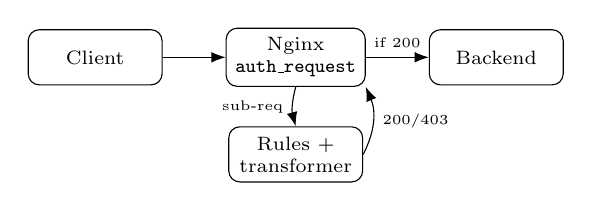
\begin{tikzpicture}[
  node distance=5mm and 8mm,
  box/.style={draw,rounded corners,align=center,minimum height=7mm,
              minimum width=17mm,font=\scriptsize},
  every edge/.style={draw,-{Latex[length=1.8mm]}}]
  \node[box] (client) {Client};
  \node[box,right=of client] (nginx) {Nginx\\\texttt{auth\_request}};
  \node[box,below=of nginx] (waf) {Rules +\\transformer};
  \node[box,right=of nginx] (app) {Backend};
  \draw (client) edge (nginx);
  \draw (nginx.south) edge[bend right=15] node[left,font=\tiny]{sub-req} (waf.north);
  \draw (waf.east) edge[bend right=25] node[right,font=\tiny]{200/403} (nginx.south east);
  \draw (nginx) edge node[above,font=\tiny]{if 200} (app);
\end{tikzpicture}
\caption{Inline enforcement via \texttt{auth\_request}.}
\label{fig:arch}
\end{figure}

\begin{algorithm}[t]
\caption{Decision fusion (Tier 4)}
\label{alg:fusion}
\begin{algorithmic}[1]
\REQUIRE $(\text{method},\text{uri})$, model score $p$, $\tau_h{=}0.98$, $\tau_\ell{=}0.90$
\STATE $u \gets \text{doubleDecode}(\text{uri})$
\IF{$\text{directSignature}(u)$} \STATE \textbf{return} \textsc{block} \ENDIF
\STATE $s \gets \text{ruleSignals}(u)$
\IF{$(s.\text{keyword} \wedge s.\text{injection}) \vee s.\text{encoding}$}
   \STATE \textbf{return} \textsc{block}
\ENDIF
\IF{$p > \tau_h \wedge s.\text{hasSignal}$} \STATE \textbf{return} \textsc{block} \ENDIF
\IF{$\tau_\ell \le p < \tau_h \wedge (s.\text{keyword} \vee s.\text{charAnom})$}
   \STATE \textbf{return} \textsc{block}
\ENDIF
\STATE \textbf{return} \textsc{allow}
\end{algorithmic}
\end{algorithm}

\section{Methodology and Setup}

\subsection{Problem formulation and preprocessing}
Detection is binary classification of $x=\texttt{METHOD}\,\Vert\,\texttt{URI}'$,
where $\texttt{URI}'$ is the request path and query after normalisation. Each
request is double URL-decoded to expose encoded payloads, contiguous digit runs
are replaced by a single placeholder token so the model does not overfit to
identifiers, and the resulting string is tokenised with the base model's
WordPiece vocabulary at a maximum length of $256$ tokens. This preprocessing is
shared between the offline evaluation and the deployed detection service, so the
two are guaranteed to agree.

\subsection{Model and training}
We fine-tune \texttt{bert-base-uncased}~\cite{devlin2019bert} with AdamW
(learning rate $2{\times}10^{-5}$, batch size $16$, weight decay $0.01$,
warmup ratio $0.1$, three epochs, early stopping on validation F1); the
training harness is model-agnostic and also supports
SecureBERT~\cite{aghaei2022securebert,aghaei2025securebert2} and
DistilBERT~\cite{sanh2019distilbert} as drop-in encoders, whose systematic
comparison we leave to future
work. Table~\ref{tab:hyperparams} summarises the training configuration and
hardware used to produce every number reported in the results below, so the
run is reproducible from these settings alone.

\begin{table}[t]
\centering
\caption{Training configuration and hardware.}
\label{tab:hyperparams}
\begin{tabular}{@{}ll@{}}
\toprule
Setting & Value \\
\midrule
Base encoder & \texttt{bert-base-uncased} \\
Max sequence length & 256 tokens \\
Optimiser & AdamW \\
Learning rate & $2\times10^{-5}$ \\
Batch size & 16 \\
Weight decay & 0.01 \\
Warmup ratio & 0.1 \\
Epochs (early-stopped on val.\ F1) & 3 \\
Random seed & 42 (fixed across runs) \\
GPU & NVIDIA Tesla T4 \\
Framework & PyTorch 2.11 (CUDA 12.8), \\
 & Hugging Face Transformers 4.x \\
\bottomrule
\end{tabular}
\end{table}

\subsection{Data and splits}
We evaluate on the CSIC~2010 tabular corpus~\cite{gimenez2010csic}, deduplicated on the normalised
request text before splitting to prevent near-duplicate benign templates from
leaking across partitions, giving $9{,}492$ unique requests ($68\%$ malicious)
split $70/15/15$ stratified by label (seed $42$), with a $1{,}424$-request held-out
test set never used for training or model selection.

\subsection{Metrics, baselines, and protocol}
We report precision, recall, F1, false-positive rate (FPR), and ROC--AUC, and
emphasise FPR because the operational cost of a WAF is dominated by wrongly
blocking legitimate users rather than by raw accuracy. Baselines are the
deterministic rule engine alone (Tiers~1--2) and TF--IDF character-$n$-gram
features with a linear SVM and a random forest. Protocols: \emph{within-dataset}
detection on the CSIC~2010 splits; \emph{ablation} evaluating rules-only,
model-only, and the full hybrid on the identical test set; \emph{threshold
sensitivity} sweeping the model's decision threshold; and \emph{adversarial}
evaluation mutating blocked payloads with six semantics-preserving
transformations. Environment: NVIDIA Tesla~T4 GPU, PyTorch~2.11 (CUDA~12.8),
Hugging Face Transformers~4.x, all seeds fixed to $42$.

\section{Results}
All figures are on the held-out CSIC~2010 test split ($n=1{,}424$).

\subsection{Detection and ablation}
Table~\ref{tab:main} and Fig.~\ref{fig:bars} report detection. The fine-tuned
BERT detector is strongest (F1~$0.966$, FPR~$0.044$, AUC~$0.986$), edging the
TF--IDF SVM on F1 and improving its false-positive rate, and far exceeding the
signature rule engine, which recalls only $43.5\%$ of attacks at a $20.9\%$
false-positive rate on this corpus. The hybrid, which blocks when \emph{either}
the rules or the model fire, inherits the rules' false positives---F1 falls to
$0.861$ and FPR rises to $0.231$---so on a benchmark whose benign traffic the
signatures were not calibrated for, the rule layer subtracts accuracy. As
Section~\ref{sec:crossdataset} shows, this is not the whole story.

\begin{table}[t]
\centering
\caption{Detection and ablation on CSIC 2010 (test). Best per column in bold.}
\label{tab:main}
\begin{tabular}{@{}lccccc@{}}
\toprule
Method & P & R & F1 & FPR & AUC \\
\midrule
Rules only            & 0.816 & 0.435 & 0.567 & 0.209 & --- \\
TF--IDF + SVM         & 0.973 & 0.957 & 0.965 & 0.057 & \textbf{0.992} \\
TF--IDF + RF          & 0.929 & 0.924 & 0.927 & 0.150 & 0.958 \\
BERT (model only)     & \textbf{0.979} & \textbf{0.953} & \textbf{0.966} & \textbf{0.044} & 0.986 \\
\textbf{Hybrid (ours)}& 0.885 & 0.837 & 0.861 & 0.231 & 0.986 \\
\bottomrule
\end{tabular}
\end{table}

\begin{figure}[t]
\centering
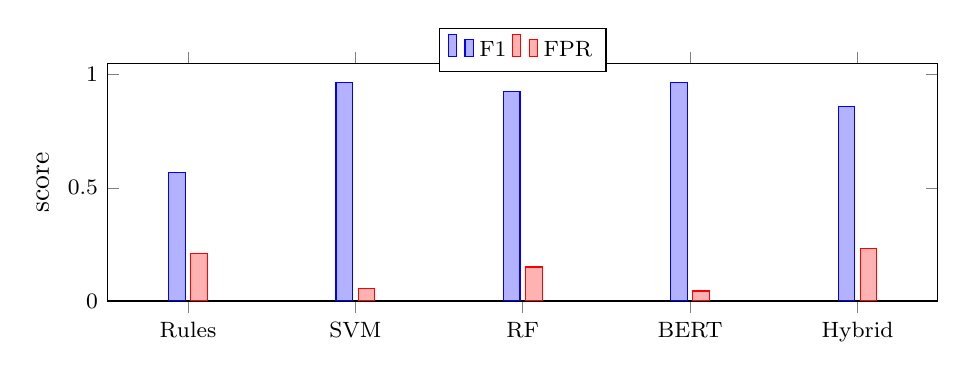
\begin{tikzpicture}
\begin{axis}[
  width=\columnwidth, height=4.6cm, ybar, bar width=6pt,
  symbolic x coords={Rules,SVM,RF,BERT,Hybrid}, xtick=data,
  ymin=0, ymax=1.05, ylabel={score},
  legend style={at={(0.5,1.15)},anchor=north,legend columns=2,font=\footnotesize},
  x tick label style={font=\footnotesize}, y tick label style={font=\footnotesize},
  enlarge x limits=0.12]
\addplot coordinates {(Rules,0.567)(SVM,0.965)(RF,0.927)(BERT,0.966)(Hybrid,0.861)};
\addplot coordinates {(Rules,0.209)(SVM,0.057)(RF,0.150)(BERT,0.044)(Hybrid,0.231)};
\legend{F1, FPR}
\end{axis}
\end{tikzpicture}
\caption{F1 and FPR by configuration on CSIC~2010.}
\label{fig:bars}
\end{figure}

\subsection{Per-attack-class recall}
Restricting to malicious test requests, the hybrid recalls SQL-injection and
encoding-style payloads perfectly ($1.00$ each) and the residual ``other''
category at $0.79$ (Fig.~\ref{fig:perclass}); the model-only configuration shows
the same ordering. Injection and encoding attacks carry strong lexical and
structural cues that both the signatures and the transformer capture, whereas the
heterogeneous ``other'' bucket---requests that do not match an obvious keyword
pattern---is hardest for both.

\begin{figure}[t]
\centering
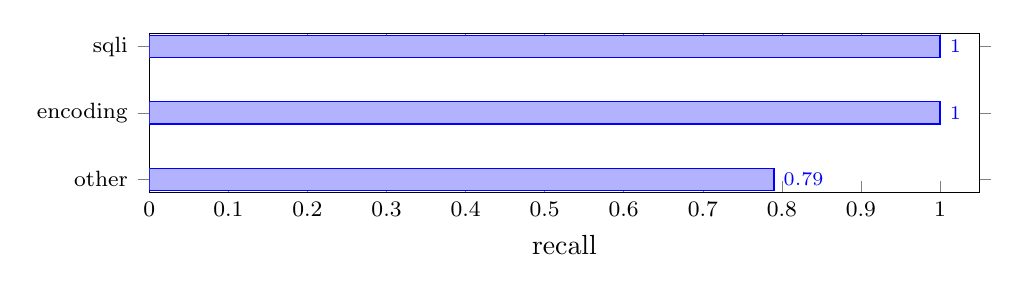
\begin{tikzpicture}
\begin{axis}[
  width=\columnwidth, height=3.6cm, xbar, bar width=8pt,
  symbolic y coords={other,encoding,sqli}, ytick=data,
  xmin=0, xmax=1.05, xlabel={recall},
  nodes near coords, nodes near coords style={font=\scriptsize},
  x tick label style={font=\footnotesize}, y tick label style={font=\footnotesize}]
\addplot coordinates {(1.0,sqli)(1.0,encoding)(0.790,other)};
\end{axis}
\end{tikzpicture}
\caption{Per-attack-class recall of the hybrid on CSIC~2010.}
\label{fig:perclass}
\end{figure}

\subsection{Threshold, latency, and adversarial robustness}
The transformer's probability lets an operator trade recall for precision: across
$\tau\in[0.50,0.98]$ recall falls from $0.953$ to $0.902$ while FPR more than
halves from $0.044$ to $0.018$ (Fig.~\ref{fig:threshold}). Single-request GPU
inference costs a median $12.0$~ms ($p99{=}17.0$~ms, ${\approx}87$~req/s per
process), fast enough for inline use. Finally, all six semantics-preserving
mutations applied to the initially blocked payloads failed to evade
\emph{either} the model alone or the hybrid ($0\%$ evasion for both,
Table~\ref{tab:latency})---unlike the model-only ML WAFs that
WAF-A-MoLE~\cite{demetrio2020wafamole} and AdvSQLi~\cite{advsqli2024} show can
be mutated past, a fine-tuned transformer on this corpus already resists these
six mutation families without help from the rule layer. Adversarial-mutation
resistance therefore does not, by itself, justify the hybrid's higher
false-positive rate; Section~\ref{sec:crossdataset} shows what does.

\begin{figure}[t]
\centering
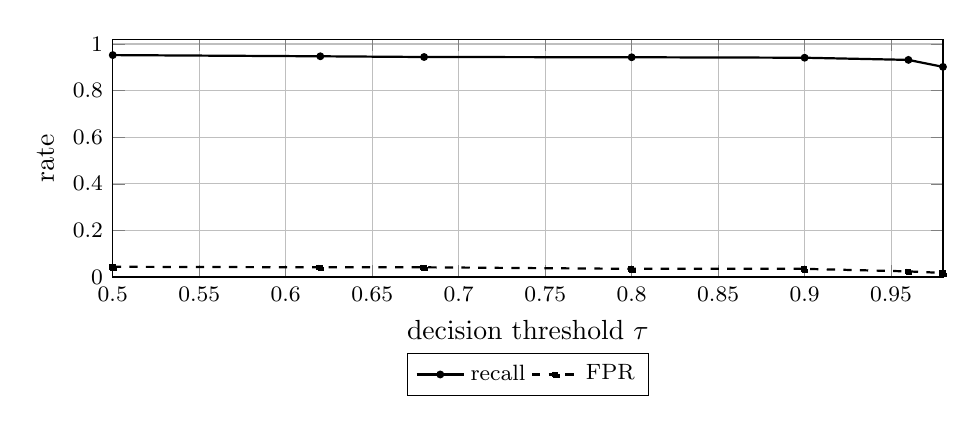
\begin{tikzpicture}
\begin{axis}[
  width=\columnwidth, height=4.6cm,
  xlabel={decision threshold $\tau$}, ylabel={rate},
  xmin=0.5, xmax=0.98, ymin=0, ymax=1.02, grid=major,
  legend style={at={(0.5,-0.32)},anchor=north,legend columns=2,font=\footnotesize},
  x tick label style={font=\footnotesize}, y tick label style={font=\footnotesize}]
\addplot[thick,mark=*,mark size=1pt] coordinates {
 (0.50,0.9525)(0.62,0.9474)(0.68,0.9443)(0.80,0.9432)(0.90,0.9412)(0.96,0.9319)(0.98,0.9020)};
\addplot[thick,dashed,mark=square*,mark size=1pt] coordinates {
 (0.50,0.0440)(0.62,0.0418)(0.68,0.0418)(0.80,0.0352)(0.90,0.0352)(0.96,0.0242)(0.98,0.0176)};
\legend{recall, FPR}
\end{axis}
\end{tikzpicture}
\caption{Recall and FPR versus decision threshold on CSIC~2010.}
\label{fig:threshold}
\end{figure}

\begin{table}[t]
\centering
\caption{Inline latency (Tesla T4) and adversarial evasion (6 mutation families).}
\label{tab:latency}
\begin{tabular}{@{}lcccc@{}}
\toprule
Config & p50 (ms) & p99 (ms) & RPS & Evasion \\
\midrule
BERT (model only) & 12.0 & 17.0 & 86.8 & 0.00 \\
Hybrid & --- & --- & --- & 0.00 \\
\bottomrule
\end{tabular}
\end{table}

\subsection{Cross-dataset generalisation}
\label{sec:crossdataset}
The results above are all within-corpus: train and test come from the same
CSIC~2010 distribution. To test what actually happens when the detector meets
traffic it was not trained on, we evaluate the CSIC-trained model zero-shot on
an independent corpus, SR-BH~2020~\cite{srbh2020}, with no retraining
(Table~\ref{tab:crossdataset}). The model alone collapses: FPR rises to
$1.00$, meaning it flags essentially all SR-BH traffic as malicious, and its
F1 falls to $0.601$ despite perfect recall. The hybrid, evaluated on the
identical SR-BH requests, recovers almost completely: FPR falls to
$0.001$ and F1 reaches $0.971$. This is the result the adversarial-evasion
test in the previous subsection could not show: the rule layer's
false-positive cost on CSIC~2010 buys back nearly all of the accuracy the
model alone loses when the traffic distribution shifts, which we take as the
strongest evidence in this paper for keeping the rule layer.

\begin{table}[t]
\centering
\caption{Zero-shot cross-dataset transfer: CSIC-trained detector on SR-BH~2020.}
\label{tab:crossdataset}
\begin{tabular}{@{}lccccc@{}}
\toprule
Configuration & P & R & F1 & FPR & AUC \\
\midrule
CSIC $\to$ CSIC (reference) & 0.979 & 0.953 & 0.966 & 0.044 & 0.986 \\
CSIC $\to$ SR-BH (model only) & 0.429 & 1.000 & 0.601 & \textbf{1.000} & 0.859 \\
CSIC $\to$ SR-BH (hybrid) & 0.999 & 0.944 & \textbf{0.971} & 0.001 & 0.859 \\
\bottomrule
\end{tabular}
\end{table}

\section{Discussion}
The central finding here is a trade-off, though not the one we set out to
find. The transformer alone turns out to be the best detector on every
accuracy metric we measured, and it resists all six mutation families we
tested just as well as the hybrid does---which was not what we expected
going in. On this evidence, adversarial-mutation robustness does not
explain why the hybrid's higher false-positive cost is worth paying. What
does explain it is distribution shift. Test the model alone on a corpus it
has never seen, and it collapses: FPR~$1.00$ on SR-BH~2020. Test the hybrid
on the exact same zero-shot data, and it holds at F1~$0.971$. The rule
layer's cost on CSIC~2010 is real (FPR climbs from $4.4\%$ to $23.1\%$), but
so is the benefit, and the benefit is invisible unless the evaluation
actually leaves the training distribution---a study confined to one corpus
will never see it. In practice, this means weighing the rule layer's
within-corpus false-positive cost against what it recovers cross-corpus,
rather than leaning on adversarial-evasion results alone. There is a
symmetry worth pointing out here too: the same rule brittleness that
motivates learned detection in the first place---signatures tuned for one
application misfiring on another, measured at $20.9\%$ FPR for rules-only on
CSIC~2010---shows up in reverse for the model, which is just as brittle once
the traffic distribution shifts. Our F1 of $0.966$ sits below the $>$99\%
figures reported elsewhere on
CSIC~2010~\cite{wadbert2026,scireports2024novelxsssqli}; we suspect this is
mostly because we deduplicate templated benign traffic before splitting,
which prevents near-duplicate leakage between train and test and gives a
stricter estimate rather than a weaker model. A few limitations are worth
naming directly. The cross-dataset test only runs in one direction---we have
not yet trained on SR-BH and tested back on CSIC---it comes from a single
fine-tuning run, and the six evasion families we tried are not exhaustive.
On scope, the detector only looks at the request line and, where present,
the body; it does not inspect responses, so we make no claim about catching
data exfiltration. The fail-open safeguard trades security for availability,
and its activation rate needs to be watched in production. Because the
evaluation code, rule engine, and preprocessing are shared verbatim with the
deployed service, every number reported here is reproducible against the
exact logic running inline.

One caveat on the latency figure in Table~\ref{tab:latency}: it is a GPU
number, and that does not mean the system needs a GPU to run. A single
Tesla~T4 handles every inline request in our test, but the same fine-tuned
\texttt{bert-base-uncased} checkpoint also runs on CPU, just slower per
request---which is exactly why the training harness treats the encoder as
swappable and already supports DistilBERT as a lighter drop-in option for
CPU-only or cost-constrained deployments. We have not benchmarked that
configuration end to end yet, so it remains an available option here rather
than a validated result. Memory-wise, the loaded model takes up a few
hundred megabytes, which is small next to typical reverse-proxy sizing and
not, by itself, a reason to rule out deployment.

\section{Threats to Validity}
\textbf{Internal.} All results come from a single fine-tuning run and a
single train/validation/test split (seed~$42$); we do not yet report
variance across seeds, so point estimates should be read with that caveat.
\textbf{Construct.} FPR and F1 on a held-out split are proxies for
operational cost and are only as good as the label quality of CSIC~2010 and
SR-BH~2020 themselves, neither of which we re-annotated. \textbf{External.}
The cross-dataset test covers one direction (CSIC-trained, SR-BH-tested);
the reverse direction and additional corpora with different traffic and
attack distributions remain future work, so the generalisation result,
while real, should not be read as covering all distribution shift.
\textbf{Adversarial scope.} The six mutation families we test are
representative, not exhaustive; a $0\%$ evasion rate against them is
evidence of robustness to that mutation family, not a general
adversarial-robustness guarantee.

\section{Conclusion}
We set out to build a WAF that puts a fine-tuned transformer inline through
Nginx's \texttt{auth\_request} mechanism and to actually measure what that
costs, rather than reporting an offline accuracy number and stopping there.
On CSIC~2010, the transformer reaches F1~$0.966$ at a $4.4\%$ false-positive
rate with $12.0$~ms median inference. Adding the rule layer costs precision
within-corpus---F1 drops to $0.861$, FPR climbs to $23.1\%$---and, contrary
to what we expected, that cost is not repaid by better resistance to
adversarial mutation, since the model alone already resists the same six
mutation families on its own. It is repaid by generalisation instead: tested
zero-shot on an independent corpus, the model alone collapses to FPR~$1.00$
while the hybrid holds at F1~$0.971$. If there is one thing worth taking
from this paper, it is that reordering: the rule layer earns its keep not
where the offline literature usually looks---adversarial mutation of known
attacks---but where that literature almost never looks at all, which is
distribution shift to traffic the model has never seen. A real deployment
needs to weigh that specific trade-off rather than assume the transformer is
sufficient on its own just because it survives mutation testing. What we
would do next: run the cross-dataset test in the other direction and
against additional corpora, benchmark a distilled encoder for CPU-only
deployment, try calibrated fusion instead of the current either/or rule,
and test adversarial training against the same mutation families evaluated
here.

\section*{Statement on the Use of AI-Assisted Tools}
Portions of this manuscript's prose --- background synthesis, drafting, and
editing --- were produced with the assistance of an AI language model
(Claude, Anthropic). The experimental design, implementation, execution,
and all reported results are the authors' own work; the authors reviewed,
verified, and take full responsibility for the accuracy and integrity of
the final text and all claims herein, consistent with this venue's policy
on AI-generated content.

\bibliographystyle{IEEEtran}
\bibliography{references}

\end{document}
